\documentclass[11pt]{article}
\usepackage[brazilian]{babel}
\usepackage[utf8]{inputenc} %acentuação da língua portuguesa
\usepackage[T1]{fontenc} 
\usepackage{wrapfig} %figura ao lado do texto
\usepackage{graphicx} %pacote de figuras

\usepackage{amsfonts} %pacote com \mathbb{}

\usepackage[pdftex]{hyperref} %links da internet

\usepackage{fancyhdr} 

\usepackage{hyphenat} %retirar hefenação

\tolerance=1 %retirar hefenação

\emergencystretch=\maxdimen %retirar hefenação

\hyphenpenalty=10000 %retirar hefenação

\hbadness=10000 %retirar hefenação

\hyphenchar\font=-1 %retirar hefenação

\sloppy %retirar hefenação

\usepackage{textcomp}

\usepackage[a4paper,left=2cm,right=2cm,top=2.5cm,bottom=2cm]{geometry}

\setlength{\parindent}{0pt} %Parágrafo sem identação]

\begin{document}
	
	\pagestyle{fancy}
	\renewcommand{\headrulewidth}{0pt}
	\renewcommand{\footrulewidth}{2.1pt}
	\fancyfoot[L]{\small Diego Silveira Costa Nascimento}
	\fancyfoot[R]{\small diego.nascimento@ifrn.edu.br}
	
	\begin{minipage}[c][1.5cm][c]{3cm}
		\begin{flushleft}
			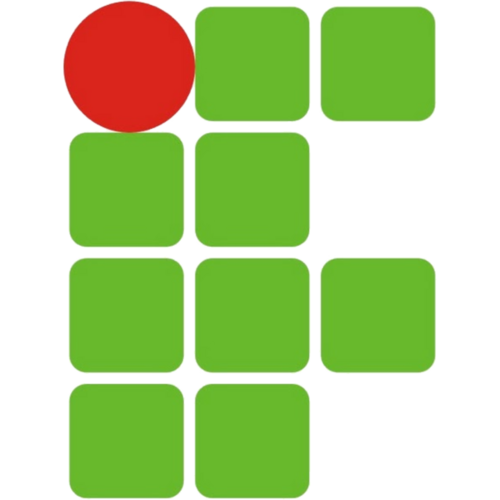
\includegraphics[scale=0.25]{IFRN}
		\end{flushleft}
	\end{minipage}		
	\begin{minipage}[c][1.5cm][c]{10.8cm}
		\begin{center}
			\resizebox{!}{0.3cm}{\textbf{Gestão Organizacional}}\par
			\resizebox{!}{0.2cm}{\textbf{Instituto Federal de Educação, Ciência e Tecnologia do Rio Grande do Norte}}\par
			\resizebox{!}{0.2cm}{\today}
		\end{center}
	\end{minipage}
	
	\begin{center}
		Exercícios
	\end{center}
	
	\section{Administra\c cão}
	
	\begin{enumerate}
		\item O que é administra\c cão?
		\item Qual a diferen\c ca entre eficácia e eficiência?
		\item Quais os principais nomes da administra\c cão clássica e suas principais contribui\c cões?
	\end{enumerate}
	
	\newpage
	\section{Estratégia}

	\begin{enumerate}
		\item O que é estratégia?
		\item Pesquise três empresas conhecidas e identifique qual a estratégia de negócio (missão, visão e valores).
		\item O que é análise de SWOT?
		\item Para as empresas pesquisadas na Questão 2, monte para cada uma delas, uma matriz de SWOT.
	\end{enumerate}	

	\newpage
	\section{Organiza\c cão}

	\begin{enumerate}
		\item O que é uma organiza\c cão?
		\item O que são metas e indicadores SMART?
		\item Estipule três metas e indicadores SMART para sua vida?
		\item O que é um quadro canva?
		\item Elabore um quadro canva para uma empresa na sua área de forma\c cão.
	\end{enumerate}	

	\newpage
	\section{Inova\c cão}

	\begin{enumerate}
		\item O que é inova\c cão?
		\item O que é Design Thinking?
		\item Desenvolva um produto ou servi\c cão inovador utilizando Design Thinking.
	\end{enumerate}

	\newpage
	\section{Gestão de tempo}

	\begin{enumerate}
		\item O que é gestão de tempo?
		\item O que é princípio da decisão de Eisenhower?
		\item Elabora uma matriz de Eisenhower para suas atividades.
	\end{enumerate}

\end{document}